\documentclass[tikz,border=10pt]{standalone}
\begin{document}
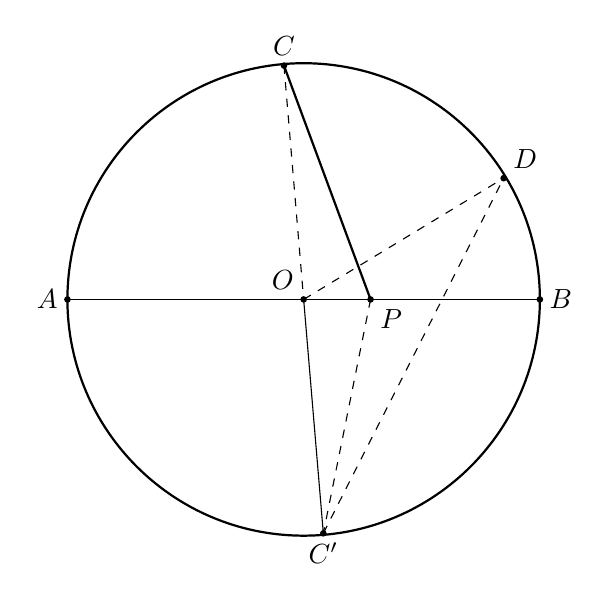
\begin{tikzpicture}
  \coordinate (O) at (0,0);
  \coordinate (A) at (-3,0);
  \coordinate (B) at (3,0);
  \coordinate (C) at (-0.25,2.97);
  \coordinate (Cp) at (0.25,-2.97);
  \coordinate (P) at (0.85,0);
  \coordinate (D) at (2.54,1.54);

  \draw[thick] (O) circle (3);
  \draw (A) -- (B);
  \draw[thick] (C) -- (P);
  \draw[dashed] (C) -- (O);
  \draw[dashed] (O) -- (D);
  \draw[dashed] (P) -- (Cp);
  \draw[dashed] (Cp) -- (D);
  \draw (O) -- (Cp);

  \node[above] at (C) {$C$};
  \node[left] at (A) {$A$};
  \node[right] at (B) {$B$};
  \node[above left] at (O) {$O$};
  \node[below right] at (P) {$P$};
  \node[above right] at (D) {$D$};
  \node[below] at (Cp) {$C'$};

  \foreach \X in {A,B,C,Cp,O,P,D}
    \fill (\X) circle (1.2pt);
\end{tikzpicture}
\end{document}
